% THIS IS SIGPROC-SP.TEX - VERSION 3.1
% WORKS WITH V3.2SP OF ACM_PROC_ARTICLE-SP.CLS
% APRIL 2009
%
% It is an example file showing how to use the 'acm_proc_article-sp.cls' V3.2SP
% LaTeX2e document class file for Conference Proceedings submissions.
% ----------------------------------------------------------------------------------------------------------------
% This .tex file (and associated .cls V3.2SP) *DOES NOT* produce:
%       1) The Permission Statement
%       2) The Conference (location) Info information
%       3) The Copyright Line with ACM data
%       4) Page numbering
% ---------------------------------------------------------------------------------------------------------------
% It is an example which *does* use the .bib file (from which the .bbl file
% is produced).
% REMEMBER HOWEVER: After having produced the .bbl file,
% and prior to final submission,
% you need to 'insert'  your .bbl file into your source .tex file so as to provide
% ONE 'self-contained' source file.
%
% Questions regarding SIGS should be sent to
% Adrienne Griscti ---> griscti@acm.org
%
% Questions/suggestions regarding the guidelines, .tex and .cls files, etc. to
% Gerald Murray ---> murray@hq.acm.org
%
% For tracking purposes - this is V3.1SP - APRIL 2009

\documentclass{style}

\usepackage{paralist}
\usepackage{graphicx}


\begin{document}

\title{Cache Oblivious B-trees}
%
% You need the command \numberofauthors to handle the 'placement
% and alignment' of the authors beneath the title.
%
% For aesthetic reasons, we recommend 'three authors at a time'
% i.e. three 'name/affiliation blocks' be placed beneath the title.
%
% NOTE: You are NOT restricted in how many 'rows' of
% "name/affiliations" may appear. We just ask that you restrict
% the number of 'columns' to three.
%
% Because of the available 'opening page real-estate'
% we ask you to refrain from putting more than six authors
% (two rows with three columns) beneath the article title.
% More than six makes the first-page appear very cluttered indeed.
%
% Use the \alignauthor commands to handle the names
% and affiliations for an 'aesthetic maximum' of six authors.
% Add names, affiliations, addresses for
% the seventh etc. author(s) as the argument for the
% \additionalauthors command.
% These 'additional authors' will be output/set for you
% without further effort on your part as the last section in
% the body of your article BEFORE References or any Appendices.

\numberofauthors{3} %  in this sample file, there are a *total*
% of EIGHT authors. SIX appear on the 'first-page' (for formatting
% reasons) and the remaining two appear in the \additionalauthors section.
%
\author{
% You can go ahead and credit any number of authors here,
% e.g. one 'row of three' or two rows (consisting of one row of three
% and a second row of one, two or three).
%
% The command \alignauthor (no curly braces needed) should
% precede each author name, affiliation/snail-mail address and
% e-mail address. Additionally, tag each line of
% affiliation/address with \affaddr, and tag the
% e-mail address with \email.
%
% 1st. author
\alignauthor
Salman Ahmad\\
\affaddr{MIT CSAIL}
\email{saahmad@mit.edu}
% 2nd. author
\alignauthor
Leilani Battle\\
\affaddr{MIT CSAIL}
\email{leibatt@mit.edu}
% 3rd. author
\alignauthor
Stephen Tu\\
\affaddr{MIT CSAIL}
\email{stephent@mit.edu}
}
% There's nothing stopping you putting the seventh, eighth, etc.
% author on the opening page (as the 'third row') but we ask,
% for aesthetic reasons that you place these 'additional authors'
% in the \additional authors block, viz.
\date{7 December 2011}
% Just remember to make sure that the TOTAL number of authors
% is the number that will appear on the first page PLUS the
% number that will appear in the \additionalauthors section.

\newcommand{\lhyperceil}{\lceil\lceil}
\newcommand{\rhyperceil}{\rceil\rceil}
\newcommand{\lhyperfloor}{\lfloor\lfloor}
\newcommand{\rhyperfloor}{\rfloor\rfloor}

\newcommand{\Search}{\textsc{Search(k)}}
\newcommand{\Insert}{\textsc{Insert(k, v)}}
\newcommand{\Scan}{\textsc{Scan(a, b)}}
\newcommand{\Delete}{\textsc{Delete(k)}}
\newcommand{\Succ}{\textsc{Succ(k)}}
\newcommand{\Pred}{\textsc{Pred(k)}}
\newcommand{\Member}{\textsc{Member(k)}}
%\newcommand{\Range}{\textsc{Range-Query(k$_{i}$,k$_{j}$)}}

\maketitle
\begin{abstract}

This paper present a survey on cache-oblivious B-trees (CO B-trees). The CO
B-tree was first introduce by Bender et al in 2000. It is an external memory
data structure - meaning that it optimizes the number of memory transfers it
performs rather than the number of CPU instructions that it executions. Unlike
other external memory data structures, like the widely use B-tree, the CO
B-tree does not require any information about the number of level in the
machine's memory hierarchy, the block size and capacity at each level, or the
relative speeds at each level. Hence, the CO B-tree is ``cache-oblivious''.
Despite this, the CO B-tree is able to achieve the same optimal search bound
as the B-tree and near optimal insertion and deletion bounds as well. In this
paper we first describe the original CO B-tree and explain how it is able to
achieve its memory performance. We then present and analyze three followup CO
B-tree data structures that improved upon shortcoming of the original: the
cache-oblivious string B-tree, which introduces support for variable length
keys, the cache-oblivious streaming B-tree, which incorporates improvements to
the insertion bound at the expense of the search bound, and lastly, the
cache-oblivious concurrent B-tree, which introduces support for concurrency.

\end{abstract}

\section{Introduction}

\subsection{External Memory Algorithms}


Most algorithms assume an idealized model of computation that consists of a
single CPU, which performs instructions, and memory, which is a flat array
that can be read and written. However, in reality memory is not a flat array
but rather a hierarchy from super fast on chip caches, to slower main memory,
to even slower disks. When a program requests data, the data is found in the
memory hierarchy and typically carried up the hierarchy to the fastest memory
layer possible, usually a cache. The CPU is then able to access it to perform
any necessary operations. Unfortunately, this cache often has a small capacity
and once it is filled any new data requests cause some existing cached data to
be evicted. Transfering data from lower to higher levels in the memory
hierarchy often takes a long time. In fact, access times between the different
layers of the hierarchy can differ by many orders of magnitude and thus the
time to transfer data often dominates the overall runtime performance of an
algorithm. External memory algorithms are wary of this fact and aim to
optimizing the number of memory transfers it performs rather than the number
of instructions it executes. They often try to exploit the fact the memory
hierarchies transfer data in blocks rather than individual atomic units. Thus,
external memory algorithms are designed to not only limit the number of memory
transfers it performs but also preserve the locality of related data so that
when a memory access is performed, its cost is amortized.

\subsection{B-trees}

Since external memory algorithms are primarily concerned with accessing data,
it is no surprise that many external memory problems can be reduced to finding
a suitable data structure that efficiently implement certain operations. A
well known external memory data structure is the B-tree. At a high level, the
B-tree works by making each one of its nodes the same size as a memory block
in a particular level of the hierarchy. Furthermore, the fanout in the tree
(the number of children of a node) is proportional to the block size as well.
The B-tree incurs $O(log(N))$ memory transfers for \Search{}, \Insert{}, and
\Delete{} and is widely used in databases and filesystems.

\subsection{DAM vs CO}

The B-tree has two theoretical shortcomings. First, the B-tree is analyzed in
a two-level memory model called the Disk Access Machine (DAM) \cite{Aggarwal}.
However, in reality, computing architectures typically have memory hierarchies
that are much larger than two. The argument for the DAM model is that in
practice only one level in the memory hierarchy tends to dominate the
performance and thus a two-level memory model is sufficient for all intents
and purposes. However, this does mean that, theoretically, B-trees can begin
to incur an increasing number of memory transfers if the dominating level in
the hierarchy changes.

Additionally, the B-tree expects to know the block size of its memory layer in
advanced. B-Trees are implemented with parameterized code that needs to be
changed for every level in the memory hierarchy. Needless to say, this tuning
can be very difficult and error prone. Additionally, tuning this parameter may
even be impossible in certain heterogeneous computing environments.

The shortcomings of the DAM model gave rise to the cache-oblivious (CO) model
of computation. In the CO model an algorithm has no information about the
memory hierarchy. It does not know anything about the speed or the block size
of any level. Conceptually, the CO model allow algorithm designers to reason
about the simple two-level model like DAM but prove results for any arbitrary
multi-level memory hierarchy. This is because algorithms that perform well in
a CO model should, in theory, perform well regardless of changes in block
size, cache capacity, and cache speed. Consequently, CO algorithm should
gracefully scale to multi-level hierarchies as well.

\subsection{CO B-trees}

In \cite{BenderDemainColton} Bender et al. introduce the cache-oblivious
B-tree (CO B-tree). The CO B-tree is similar to the normal B-tree except that
it does not require explicit parameters about the memory hierarch.

The CO B-tree is able to achieve the optimal search bound of $\Theta(log(N))$
memory transfers, the optimal scan bound of $\Theta(N/B)$ memory transfers and
near optimal insertion and deletion bound of $\Theta(log_B N +
\frac{log^2{N}}{B})$. The CO B-tree was a seminal data structure that gave
rise to many others.

This paper provides a survey of the different types of CO B-trees and
discusses the various trade offs that they make. We start by analyzing the
original CO B-tree and explain how it works. This includes a detailed
description of the packed memory array (PMA) and strongly weight-balance
binary search trees (SWSBT) that are integral to the CO B-tree's memory
performance. Following this discussion we provide an analysis of the CO String
B-tree,a CO B-tree with variable length keys, the CO Streaming B-tree, a CO
B-tree that improves the cost of insertion at the expense of search, and the
CO Concurrent B-tree, which allows multiple processes to access the data at
the same time.

\section{Background}




High level idea:

We want to have a B-tree that is cache oblivious. Okay, well, first we still
need a way to actually store our data. We should use a tree. But what type of
tree? Obviously it needs to be balanced but anything else? Yes, it needs to
maintain the property that the number of descendants are $O(d^h)$. Why? It has
to do with how we will ultimately layout the tree in memory, but we will get
to that later.

Okay, so, we find the tree that we want to use. Now what? Well, first of all,
we need to make sure that it supports all of the operations that we want while
maintain this key property. Lets start with searching. We will layout the tree
in a vEB layout. This is helpful for two reasons. First, it is a nice way to
store it in memory and second because it gives us a search bound for free. Now
we need to make sure that it supports all of the other operations while
maintain the key property. I can show you how it handles insertions and
delete. Bam!

Okay, so now, we have a data structure that holds the amount of memory that we
want and it has the property that we will use later. Great! Now what? Well, we
need to actually store this in memory some how. We said that we will use a vEB
layout but that is only half of the story. We want a data structure that
maintain the locality of as many elements as once while also keeping extra
space to allow for future inserts. This is seemingly contradictory but we can
do it!

How? we use a PMA. The main problem is what inserts and delete may cause
splits and merges which may cause huge parts and nodes of the tree to move
around. So we need to first show how it is able to handle splits and merges
efficiently in a cache oblivious manner. bam! done! Great!

Now what? We also have the problem of updating pointers. If the points are
close to one anther that is not a big deal. However, it is possible that the
nodes are really far apart. Close means they are in the same block and thus
only incur a single memory transfer. Far apart means they are more. To solve
this problem we use buffer nodes and that works in a weird way. However, this
only gives us a bad bound, can we do better? ****

Yes! We use indirection. Indirection allows us to use another array and this
makes out pointer updates much more efficient.

We can now perform inserts and deletions faster. Additionally, our scans are
super fast as well. Search have not changed at all because we still have our
vEB structure and thus we are okay. But, we can also do a little better. If we
are okay without having scans, we can improve inserts and deletion since we no
longer have to maintain our indirection array.

The important part is that our analysis above we never treat the block size as
a constant. It is always a variable in our analysis but we are able to achieve
the desired bounds. Thus, we have a cache-oblivious B-tree that does
everything that we want.















\subsection{Original CO B-trees}
\label{sec:original}

Bender et al. first introduced a cache oblivious B-tree (CO B-tree) in
\cite{cobtree}. The CO B-tree was able to match the optimum search bound of
$\Theta(log_B N)$ memory transfers without including any specific
parameterization describing the speed or sizes of the machine's memory
hierarchy.

The CO B-tree paper presents three different data structures that make
different trade off in the number of memory transfer they perform. However,
all of them achieve their performance by structuring their elements as a
strongly weight-balanced search tree (SWBST). The SWBST is then laid out into
a packed memory array (PMA) using a van Emde Boas (vEB) layout. The SWBST and
PMA play crucial roles in the other cache-oblivious data structures that were
developed after the CO B-tree and thus are described at length in the next two
sections.

\subsection{Structure - SWBST}
\label{sec:structure}

Strongly weight-balanced search trees play a key role in CO B-tree. The weight
of a node is $u$ is equal to the total number of $u$'s descendants plus 1. It
can als be thought of as the sum of the weights of $u$'s children plus 1.
Formally, $u$'s weight is: $w(u) = 1 + \sum_{v \in children} w(v)$.

Most weight-balanced search trees which requires that the heights of a node's
left and right subtrees are simply off by a constant factor. SWBST enforce the
stronger property that a node at height $h$ in the tree (height is the node's
distance from the leaves; leaves have a height of 1) has $\Theta c^h$ where
$c$ is some constant.

A known data structure that achieves this property is the ``weight-balanced
B-tree'' \cite{paper}. The CO B-tree leverages this data structure to maintain
its elements. The next section describes how SWBST perform various operations
while maintain their strongly weight-balanced property.

\subsection{Operations}

The CO B-tree supports \Search, \Insert, \Delete, and \Scan operations. 

\subsection{Complexity}



It should be noted, that keeping the level of indirection sorted is only
needed in case we want to perform \Scan operations. If we do not need \Scan,
then we can keep the indirection array in any arbitrary order reducing the
cost of \Insert and \Delete by the $(log^2 N) /B$ factor making them incur
$O(log_{B} N)$ memory transfers overall.

\subsection{Layout - PMA}
\label{sec:layout}

SWBST is only one half of the CO B-tree story...

\begin{figure}

\begin{center}
	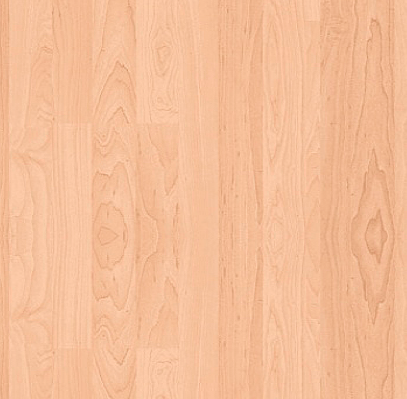
\includegraphics[width=0.8\columnwidth]{figures/veb.png}
\end{center}

\caption{An illustration of the van Emde Boas (vEB) layout}
\label{fig:veb}
\end{figure}


\section{Variable Length Strings}

\subsection{Motivation}
In order for B-trees to remain versatile, they must be able to accommodate various forms of data. However, traditional B-trees and string B-trees have suboptimal performance when variable length strings are used as keys. In \cite{BenderFaKu06}, Bender et al. describe 4 major issues:
\begin{itemize}
\item B-trees handle variable length keys poorly
\item string B-trees do not support compression, and the front compression used in many other B-trees is handled sub-optimally
\item range queries are handled sub-optimally by regular B-trees, since they result in random disk seeks
\item traditional and string B-trees assume fixed block-transfer size B at all levels of the memory hierarchy, resulting in sub-optimal performance over hierarchies with varied block-transfer sizes.
\end{itemize}
\subsection{Description}
They address these issues by designing a Cache Oblivious String B-tree.

\subsubsection{General COSB-tree Structure}
The static COSB-tree consists of 2 layers: a centroid tree at the top, and an array of the keys stored in lexicographic order on the bottom. The leaves of the centroid tree contain pointers to keys in the array. The centroid tree is structured such that a search through the centroid tree identifies the local area of the desired key in the array. Then a sequential scan is performed across the array to find the key.

The Dynamic COSB-tree consists of 3 major components: a centroid tree at the top; a packed memory array (PMA) structure of hash data for the keys known as the \emph{hashdata} layer; and on the bottom a PMA structure for the original key values, compressed using an augmented version of forward compression known as the \emph{keydata} layer.

The centroid tree on a high level behaves similarly for static and dynamic COSB-trees. The leaves of the centroid tree point into the hashdata layer, where a sequential scan is performed to find the correct key by hash value. The hashdata layer points directly into the keydata layer, where the appropriate key is decoded, compared and returned.

In the following subsections, centroid trees are explained, and a summary of how to modify them to preserve weight balance in the dynamic case is provided. Two iterations on forward compression are also summarized to show how to incrementally add support for variable length strings as keys for dynamic COSB-trees. Lastly, the design and use of the hashdata and keydata are explained.

\subsubsection{The Dictionary Matching Problem and Centroid Trees} %todo:cite dictionary matching problem--sources in cosb-tree paper
In this approach to solving the dictionary matching problem, a dictionary $D$ of $N$ keys is preprocessed using hashing and divide-and-conquer via the construction of a centroid tree over the keys. This technique forms the basis for the Cache Oblivious String B-tree (COSB-tree) design. Consider the compacted trie $T$ of $D$. Bender et al. observe that there exists a centroid vertex $\rho$ in $T$ such that $\rho$ has between N/3 and 2N/3 descendants, inclusive. When searching for a key $k$ in the compacted trie, you traverse the tree as follows: for each node $y$ that you visit, if $y$ is a prefix of $x$, or $y$ matches $x$, continue on into the trie rooted at $y$ or \emph{down trie} of $y$. Otherwise traverse the trie resulting from excluding $y$ and its subtree. The \emph{centroid tree} is obtained by rooting the tree at \emph{centroid vertex} $\rho$, and making its children recursively defined \emph{centroid trees} of its up and down tries. 

At each step through the centroid tree, a consistent fraction of the nodes are eliminated from the search, resulting in an $O(logN)$ time bound when ignoring the time required to operate on keys. To make key comparisons faster, the keys are hashed and hash values are compared in place of the original key values. To avoid mismatches due to overlap in hash values, the original key values are compared after finding a match in hash values. The resulting time bound for \Search{} (interchangeable with \Member{}) is $O(||k||+logN)$. If each node in the centroid tree knows its successor and predecessor descendants, \Pred{} and \Succ{} can be achieved in $O(||k||+||k'||+logN)$, where $k'$ is the successor or predecessor of $k$. Note that the additive $logN$ incurred by the use of centroid trees can be avoided when using main memory. Centroid trees are used to capitalize on locality for the cache oblivious string B-tree design, described later in this section.

For COSB-trees, the centroid tree is built using $O(N/logN)$ keys, and the centroid tree is layed out in memory using a modified van Emde Boas (vEB) layout for weight-balanced binary trees. The \emph{hyperhyperfloors} of nodes are used as a guide for cutting the tree into equal-size subtrees for the vEB layout. The \emph{hyperhyperfloor} of x is denoted as $\lhyperfloor{}x\rhyperfloor{}$, and refers to rounding x down to the nearest power of a power of 2. This ensures trees of equal size on all \emph{levels of detail}, as the centroid tree is traversed.

\subsubsection{Modifying Front Compression to Preserve Locality}
This section provides a brief summary of how front compression is modified to optimize compression and decoding for static and dynamic cache-oblivious string B-trees. Consider a sequence of $j$ keys to store $k_{1}$,  $k_{2}$, ...,  $k_{j}$. Without compression, this requires $\sum_{j}||k_{j}||$ space in memory. To compress these keys using front compression, let $\pi_{j}$ be the longest common prefix between $k_{j}$ and $k_{j+1}$. Now instead we store the keys as follows: 
\begin{center}
$k_{1}$,$||\pi_{2}||$,$\sigma_{2}$,$||\pi_{3}||$$\sigma_{3}$,...,$||\pi_{j}||$,$\sigma_{j}$
\end{center}
where $\sigma_{j}$ is the suffix of $k_{j}$ after removing the first $\pi_{j}$ bits. This saves almost $\sum_{j}||\pi_{j}||$ memory. However, since decoding $k_{j}$ involves concatenating the first $\pi_{j}$ bits of $k_{j-1}$ to $\sigma_{j}$, $k_{j-1}$ must be decoded. $k_{j-1}$ may depend on previous keys as well, making $k_{j}$ expensive to decode.

The goal of modifying front compression is to maintain some of the space benefits to compression while reducing the high decoding cost and keeping the size of D small. Bender et al.  provide a modification that reduces the high decoding cost of front compression of D to $O(1+||k||B)$, with size $O(\ll{D}\gg)$ after compression. The modification works as follows: Let $c = 2 + \epsilon/2$, and let $k_{1}$ be the first key added to the compression stream. For each subsequent key $k_{i}$, if $k_{i}$ can be decoded with just the last $c||k_{i}||$ characters, add $\pi_{i}$,$\sigma_{i}$ like before. Otherwise, add 0,$k_{i}$, which means add $k_{i}$ to the stream in its uncompressed form. By construction, this scheme guarantees that any key $k_{j}$ can be decoded in $O(1+||k||B)$ memory transfers.%todo: add something about why this isO(<<D>>)?
%todo: add another paragraph or two about the second iteration
\subsection{Operators}
The operations supported are

\subsection{Complexity}

\section{Streaming B-trees}

\subsection{Description}

While B-trees achieve good performance for searches, they do not perform as
well for updates and insertions. The buffered-repository tree (BRT) is a
common alternative to the B-tree achieves an improved amortized $O(log(N)/B)$
memory transfers for inserts compared to the $O(log_{B+1}N)$ memory access of
B-trees.

The search vs insertion trade off also exists in the cache-oblivious model.
The original cache-oblivious B-trees described in Section~\ref{sec:original}
achieves the search end of this trade off. However, Bender et al. propose two
data structures that and achieve the opposite end: the shuttle tree and the
cache-oblivious lookahead array (COLA) \cite{BenderFaFi07}. These two data
structures are refereed to as ``streaming B-trees'', indicating how they are
optimized for insertions at the cost of search.

\subsection{Shuttle Trees}

The shuttle tree is similar in layout and structure as the original CO B-Tree.
It uses a strongly weight-balanced search tree described previously (see
Section~\ref{sec:structure}) that is laid out in a vEB layout into a PMA. A
notable difference is that the CO B-tree splits the tree at height $h/2$ when
creating the vEB layout while the shuttle tree splits at height $F_k$ where
$F_k$ is the $kth$ Fibonacci number that is stickily less than the height of
the tree. Thus if a tree's height happens to be a Fibonacci number, $F_k$,
then the shuttle tree will choose to split the tree at height $F_{k-1}$. The
top and bottom ``halves'' produced by this split are organized just like
before and shown in Figure \ref{fig:veb}.

\begin{figure}

\begin{center}
	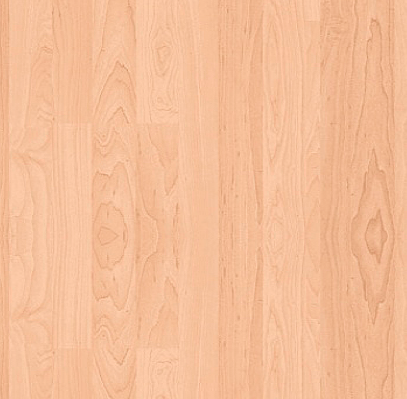
\includegraphics[width=0.8\columnwidth]{figures/veb.png}
\end{center}

\caption{An illustration of how the shuttle tree determines the size of a node's linked list}
\label{fig:buffers}
\end{figure}


The shuttle tree improves the efficiency of insertion by adding buffers to
each node in the tree. In fact, shuttle tree nodes have a linked list of
buffers rather than a single buffer like BRT and each of these buffers is
another shuttle tree. The length of a node's linked list is related to the
node's height in the tree. A node has a buffer for every time it the leaf of a
sub trees that is split when creating the vEB layout. This idea is illustrated
in Figure \ref{fig:buffers}.

The shuttle tree's node's buffers have a maximum capacity that is enforced by
bounding it height. The size of the buffers increases going across the linked
list. Thus, a node's first buffer is smaller than its last buffer. The maximum
height of a buffer is given by $F_{H(k)} = F_{k-2 \lceil log_{\phi} k \rceil}
$ where $\phi$ is the golden ratio and $k$ is chosen such that $F_k$ =
$\xi(h)$ and $\xi(x)$ is defined recursively. If $h$ is a Fibonacci number
then $\xi(h) = h$ and otherwise $\xi(h) = \xi(h-f)$ where f is the largest
Fibonacci number less than $h$. The size of the buffer is related to the size
of the recursive subtree for which the node is a leaf. Since the recursive
subtrees are split based on the largest Fibonacci number less than $h$ it
follows that the buffer sizes are also based on Fibonacci numbers.

\subsubsection{Operators}

The operations that are described by Bender et al. for the shuttle tree are
\Search, \Insert, and \Scan. An explicit discussion on \Delete is missing;
however, it is assumed that it is symmetric to \Insert.

\Search and \Scan work virtually the same way as the CO B-tree. The only
difference is that you have to search a child node's buffer before following
the pointer down the tree.

\Insert is also similar to the CO B-tree except you buffer elements as you add
new elments. When you insert an element you move down the tree from the root
to leaves and stop when you find a node that has a buffer (it is possible that
a node does not have any buffers because of the height of the tree). You then
attempt to insert the element into the smallest buffer in the node's linked
list. If this insertion causes the buffer to overflow (e.g. the height of the
buffer exceeds its maximum), you move all of the elements from this buffer to
the next largest buffer. When the largest buffer overflows you take all of its
elements and ``shuttle'' them down the tree. Eventually you will hit a leaf
node and inserting here may cause the balance constraints on the SWBST to
become invalidated. The shuttle tree rebalances itself just like any other
SWBST: the leaf node is split into two and this cascades up the tree until
balance is restored.

When a node $u$ is split into two nodes $u1$ and $u2$ we immediately allocate
enough space for all of the $u2$'s buffers. We then scan over $u$'s buffered
sub trees and find the ones rooted in $u1$ and $u2$ and move them
respectively. This can be achieved by a single scan. Once we have found the
set of subtrees that correspond to $u1$ and $u2$ we replace the original sub
trees for $u$ in the vEB layout.

The core problem of maintain room for inserts in the shuttle tree does not
change from the CO B-tree and is handled by the PMA just like in described in
Section~\ref{sec:layout}.

\subsubsection{Complexity}

The complexity of \Search is $O(log_B N)$ where $N = \Theta(c^{F_k})$ and $c$
is your fanout. Note that $c$ is not treated as a constant since this is a
cache-oblivious data structure. This bound is achieved by searching over the
top and bottom recursive subtrees at each level. A key trick is that when you
visit a node you only search its largest buffer (that last buffer in the
linked list). The smaller buffers will be visited eventually as you recurse
down the tree. Eventually you will get down to a single subtree that can fit
into $O(1)$ blocks and thus can be search with $O(1)$ memory accesses. Since
the fanout is proportional to our block size it will take us $O(log_B N)$
block accesses until we get down to a subtree and thus, by induction, the
worst case runtime is $O(log_B N)$.

\Insert uses $O(log_{B+1} N / B^{\Theta(1/(loglogB)^2)} + (log^2 N) / B)$
memory transfers. This improvement of the the CO B-tree is achieved because
the shuttle tree's buffers are used to maintain locality of the elements long
enough to amortize the cost of moving them down the tree and possible into
another block. The proof is based on the fact that when we move an item from
one block to another, caused by splitting or buffers being overfilled, at
least $B^{\Theta(1/(loglogB)^2)}$ will move with that item. This is because,
with insert, when a buffer overflows we move all of the elements from that
buffer down the tree, not just the single one that caused the overflow. Thus,
we amortize the cost of a single insert by the number of elements in a node's
largest buffer.

The complexity to \Scan $L$ elements is amortized to $O(L/B)$ memory
transfers. First you perform a \Search to get to the starting element of your
range. Once you have a block in memory you can start scanning in elements and
since you only have to read a new block every $B$ accesses each element access
is amortized to $1/B$ and thus overall the number of memory access is
$O(L/B)$. This, of course, assumes that you just performed a search for the
starting point of your scan.

The last thing that should be considered is the space requirement of the
shuttle tree. However, the overall space requirements of the shuttle tree is
actually just $O(n)$. The high level intuition for this proof is that the
majority of the buffers are really small and thus do not impact the overall
size of the tree.

\subsection{COLA}

The cache-oblivious lookahead array (COLA) is a cache-oblivious dictionary
that is actually quite different from the other cache-oblivious data
structures seen so far. Instead of an explicit tree structure with child and
parent pointers, the COLA is organized as a list of arrays or levels. Each
level has arrays of size $2^k$. Each level is either completely full or
completely empty. As such, the COLA is very similar to the binomial list
structure described in \cite{BentleySaxe}.

\subsubsection{Operators}

The operations supported by COLA are \Search, \Insert, and \Scan.

\Insert works by initially inserting the element into the first-level array.
This array has size $2^0 = 1$, thus the element is in an array on it own.
Whenever you insert an element you check to see if there is another list of
the same size and merge them together in sorted order. This merging will
produce a new array of twice the size which goes into the next level. We
continue to merge until there are no two arrays of the same length.

\Search can naively be performed by simply scanning each of the levels in our
data structure. Since everything is sorted we can use a binary search to
quickly find the element we are looking for. Obviously this is not very
efficient, thus COLA, as the name suggest, uses look ahead pointers to reduce
the number of memory accesses required. Every 8th element from the $k+1$ level
exists in the $k$ level array in its proper sorted location. This element also
contains a pointer to its real location in the $k+1$ level, thus it is
referred to as a ``real lookahead pointer''. Additionally, each every 4th cell
in $k$ level array contains two pointers pointing to the next and previous
``real lookahead pointers'' on this level. Therefore, to search a level we
perform a binary search and automatically cascade up to the next level.

\subsubsection{Complexity}

The complexity of \Insert is amortized to $O(log N / B)$ block transfers.
First, it is important to know that an element will never be merged more than
$O(log(N))$ times since at that point, it will be in the last array. The first
$log(B)$ merges that a element participates is constant time since we can
assume that the relevant blocks are already in memory. Thus, we only need to
worry about memory accesses when we merge levels that have size greater than
$B$. If the size of the array is $k$ then the cost of merging is $O(k/B)$ and
thus the amortized cost of a merging a single element is simply $1/B$. Since
an element will only be merged $log(N)$ time, the overall cost is amortized to
$O(logN/B)$.

The complexity of \Search is $O(log N)$ memory transfers. The proof is based
on the fact that we only ever need to search at most eight items on each
level. Since there are $O(log(N))$ levels and since eight is a constant it
follows that overall, search accesses $O(log N)$ blocks. A proof by induction
shows that only eight items need to be searched on each level. The base case
is trivial. The first three levels of the COLA each have at most eight
elements that either contain the actual elements or a look ahead pointer to
the next level. Obviously we can search these levels with no more than eight
member transfers. As we follow the lookahead pointers to the high levels we
will eventual get to a level where $k \geq 3$. Note that we do not enter this
level at the start; rather, we arrived here by following the real lookahead
pointers from the levels below and are at some index $i$ that contains an
element $e_i$ such that $e_i < e$ where $e$ is the element we are looking for.
Our goal is to find a new $i$ such that $e_i \leq e < e_{i+1}$. Once we find
this $i$ then we can use the duplicate look ahead pointer to find the ``next''
and previous look ahead pointers in the next level and restrict our search to
that range. Since we have a real look ahead pointer for every eighth element
in the next level, it follow that when we get to the next level, we only need
to search eight elements. Furthermore, since we arrived at our current level
from a lower level, we only need to search $8$ elements to find this $i$.
Thus, overall, we only need to perform $O(8log(N)) = O(log(N))$ memory
transfers.

\subsubsection{Performance}

In experimental results, COLA achieved significant improvements for random
inserts, performing 790 times faster than a normal B-tree. Sorted inserts are
3.1 times slower and searches are 3.5 times slower. These experimental results
indicate that the the COLA is a suitable data structure for streaming data
structure where random insertions are common.

\section{Concurrency}

\subsection{Motivation}
B-trees are often used as an indexing data structure for various
database and file systems. Thus, for a cache-oblivious B-tree data structure
to be of practical value, it must be able to handle concurrent access and modification
of its internal state. The straw-man solution is to simply ensure mutual exclusion
on the entire data structure; this approach, however, yields poor performance.

Various concurrency schemes for traditional cache-aware B-trees have been
proposed \cite{BayerS77, LehmanY81}. We now survey a concurrency scheme for CO
B-trees, first presented in \cite{BenderFiGi05}. Bender develops two different
data structures to solve this problem: the first is an exponential CO B-tree,
the second is a CO B-tree based on a packed memory array (PMA). Bender
also presents a lock-free variant of the latter data structure. For
the remainder of the discussion, assume that the keys are fixed-size integer
keys.

\subsection{Description}
Before describing the data structures in more detail, we first consider
the concurrency model which is used throughout \cite{BenderFiGi05}.

\subsubsection{Concurrency Model}
The concurrency model starts with a system that has a total cache
size of $M$ and block size of $B$. There are $P$ processors in the
system, each with a cache of size $\frac{M}{P}$. A particular block
can reside in multiple caches in \textit{shared} mode. However, if a
processor wants to perform a write to a block, it must acquire it in 
\textit{exclusive} mode, in which case that block can only reside in
a single cache. In this model, a request for a block costs a single
memory transfer.

For concurrency control, two primitives are used. The first is
locks. The second is \textit{load-linked/store-conditional} (LL/SC).
The authors argue that LL/SC provides better performance than 
using a \textit{compare-and-swap} (CAS) primitive, but their 
techniques can be extended to use CAS.

\subsection{Exponential CO B-tree}
This data structure is based on a strongly weight-balanced 
exponential tree found in \cite{Bender2002}. A tuning parameter
$1 < \alpha < 2$ is chosen for the data structure. Each node
in the tree maintains both keys which divide up its children,
in addition to a \textit{right-link} pointer, which contains
both a pointer to a node's right sibling, plus the key
value of the minimum key in the node's right sibling. If no such
sibling exists, a sentinel $\infty$ pointer is used.

A node's layout in memory is as follows. Suppose a node has $k$
elements in it. The first part of the node consists of a static
CO search B-tree, containing the $k$ elements. The tree is sized
to be a complete $\lhyperceil k \rhyperceil$-leaf tree. The second
part of the node consists of a $\lhyperceil k \rhyperceil$-size array
contained the $k$ elements in sorted order. The leaf nodes of the
CO search tree point to the associated entries in the array.

\subsubsection{Operations}
The operations supported by the exponential CO B-tree are \Search{}
and \Insert{}. The authors do not discuss range-queries, and this
is presumably due to the concurrency issues in implementing a fully-consistent
range scan (weakly-consistent range scans could be implemented in the data
structure with very little modification), although interestingly enough
the PMA variant of B-tree (discussed in Section \ref{sec:pma}) does
cover range scans. 

\Search{} works as follows. For a non-leaf node, first check the
\textit{right-link} key. If the \textit{right-link} key is less than
$k$, then traverse the right link, and recurse. Otherwise, follow
the appropriate child pointer. When a leaf node is reached, only
follow \textit{right-link} pointers, until either $k$ has been located
or some element greater than $k$ is reached. No locks are acquired
during the entire search operation.

\Insert{} works as follows. First, \Search{} is used to locate the leaf node
where $k$ will be inserted into. A lock is acquired on that node, $k$ is
inserted, and the lock is released. Unlike a standard B-tree, there is no
maximum number of elements in a node; instead we split nodes probabilistically.
With probability ${1}/{2^{\alpha^h}}$, a node at height $h$ is split (leaf
nodes have $h = 0$). A split works as follows.  We reacquire a lock on the node
to be split. We split the node into $u$ and $u'$, where $u$ contains all the
keys $< k$, and $u'$ contains the keys $\geq k$. We release the lock, and
recursively insert $k$ into the parent of the split node. It is important
to note that, since $u$ contains a prefix of the original node to be split,
that we reuse the original node in constructing $u$ (that way, concurrent
searches can still locate the keys in $u$).

%TODO: some section about linearizability?

\subsubsection{Complexity}
Sequential search takes $O(\log_B{N} + \log_{\alpha}{\log_2{B}})$ block
transfers (with high probability). The probabilistic bound comes from the
probabilistic key promotion property. The intuition behind the proof of this
bound comes from the argument that when the tree has height $h =
\Omega(\log_{\alpha}{\log_2{\log_2{N}}})$, then the total number of keys in the
tree is $O(2^{\alpha^h})$. The proof is then completed by summing over the
range of $h$ which is probabilistic $O(\log_{\alpha}{\log_2{N}})$, the access
time from some level $h$ to find the correct child.

Sequential insert takes $O(\log_B{N} + \log{\alpha}{\log_2{B}})$ block
transfers (in expectation). This proof is constructed in a similar 
fashion as the search proof: consider inserting a tree at some height $h$.
By noting that the probability a particular node reaches height $h$
is $2^{-(\alpha^h-1)/(\alpha-1)}$, a summation over all levels
of the cost of rebuilding a node yields the time-bound.

\subsection{Packed Memory Array CO B-tree}
\label{sec:pma}
The PMA CO B-tree is a two level data structure, containing a static
CO B-tree which indexes into a packed-memory array. Bender introduces
a new packed-memory array, called a \textit{one-way packed-memory array},
which they argue is easier to manage concurrently.

\subsubsection{One-Way PMA Primer}

A one-way packed-memory array is a contiguous memory structure which has three
distinct regions: a leftmost region of empty space, an \textit{active region}
which contains the elements of the array, and a rightmost region of empty
space. The array only grows into the rightmost region, and shrinks from the
leftmost region (hence one-way).  The PMA is of size $m = \Theta(N)$, subject
to $m$ being a power of $2$, where $N$ is the number of elements.

When the \textit{active region} becomes too large/small due to inserts/deletes,
the PMA is rebalanced. A new array is allocated, and the elements are
spread out evenly over the new array (too minimize element density).

Each leaf in the static CO B-tree used is a pointer into a $\Theta(\log
N)$-size region in the packed-memory array. 

\subsubsection{Operations}

\Search{} works as follows. Search the static tree for $k$ until
a leaf node is reached. Follow the leaf node pointer into the PMA.
Scan right in the PMA until either $k$ is located, or some element
$> k$ is reached. Do not acquire any locks during the search.

\Insert{} works as follows. Use \Search{} to locate the $\Theta(\log N)$-region
of the PMA which (would) contain $k$. Lock the region, and scan right to find
the appropriate slot $s$ to place $k$ into. $s$ is defined such that slot $s -
1$ contains the largest key smaller than $k$. If scanning forward requires
going into the next $\Theta(\log N)$-region, lock the next region and release
the current region (\textit{hand-over-hand} locking technique). Once $s$
is located, either $s$ is free, in which case just insert $k$, or $s$ is not free,
in which case a \textit{rebalance} operation is required.

To do a rebalance operation, we scan right (locking as necessary) until the
region from $s$ to the current position $s'$ is not \textit{too dense}. The
notion of density is defined in detail in \cite{BenderFiGi05}. The region
$[s, s']$ is then rebalanced as follows. Start from the rightmost element,
and move elements to the right (maintaining order) such that no suffix of
$[s, s']$ is too dense. This rebalancing creates room for $k$; we insert $k$
and then release the locks.

\subsubsection{Complexity}

% TODO: can somebody check this time-bound? seems kind of bad
Sequential search time-bounds are not presented in the paper,
but presumably since search is a static CO tree lookup followed
by a scan, the time bound is $O(\log_{B}{N} + {\log_2{N}}/{B} + 1)$.

Sequential insert is $O(\log_{B}{N} + \log_2^2{N}/{B} + 1)$. The proof
is based off an accounting argument which places $\Theta(\log_2^2{m}/B)$
dollars in each array slot. The proof is not presented in any detail in the
paper, but rather it is a slightly-modified version of the proof presented
in \cite{Katriel02}. 

\subsubsection{Lock-free Variant}
The lock-free variant is based on the PMA CO tree, except the locks acquired
during the PMA modification are replaced by augmenting each element in the PMA
with a marker. A marker is used to denote the ongoing (concurrent) operation
of a particular cell.

In addition, four non-blocking primitives are introduced:
\begin{inparaenum}[(a)]
  \item \textit{move},
  \item \textit{cell-insertion},
  \item \textit{cell-deletion}, and
  \item \textit{read}
\end{inparaenum}. These primitives are self-explanatory, except they
all work in a non-blocking manner (they can fail at any point).

The concurrency protocol works as follows. Any of the non-blocking primitives
are initiated by denoting the cell in question with the marker. If a process
ever encounters a cell with a marker, it drops what it is doing and first helps
to complete the operation. When the originating process gets context-switched
back in, any SCs will fail, and then the process can check to see if the
operation was already completed. The implementation of the non-blocking
primitives is spelled out in more detail in \cite{BenderFiGi05}, but the basic
idea is using LL/SC to detect when concurrent operations are on-going.

\subsubsection{Lock-free Variant Operations}

\Search{} is un-modified from the lock-based version.

\Insert{} is modified as follows. Cell $s$ is located as before. A
\textit{cell-insertion} operation is performed on $s$. If it succeeds, we are
done. If it fails, then a rebalance is necessary. Rebalance proceeds as before,
scanning right to find the region $[s, s']$. However, whenever a non-empty cell
is encountered, a load-link (LL) is performed on the cell.  Once the region is
found, the rebalancing-to-the-right is performed as before.  However, a
store-conditional (SC) is performed on the destination of each cell.  If any SC
fails, then this means concurrent modification had occurred, in which case the
algorithm restarts from the beginning.

\section{Conclusion}

%\end{document}  % This is where a 'short' article might terminate

%ACKNOWLEDGMENTS are optional
\section{Acknowledgments}
Thanks Karger

%
% The following two commands are all you need in the
% initial runs of your .tex file to
% produce the bibliography for the citations in your paper.
\bibliographystyle{abbrv}
\bibliography{citations}  % sigproc.bib is the name of the Bibliography in this case
% You must have a proper ".bib" file
%  and remember to run:
% latex bibtex latex latex
% to resolve all references
%
% ACM needs 'a single self-contained file'!
%
%APPENDICES are optional
%\balancecolumns
%\appendix
%%Appendix A
%\section{Headings in Appendices}
%The rules about hierarchical headings discussed above for
%the body of the article are different in the appendices.
%In the \textbf{appendix} environment, the command
%\textbf{section} is used to
%indicate the start of each Appendix, with alphabetic order
%designation (i.e. the first is A, the second B, etc.) and
%a title (if you include one).  So, if you need
%hierarchical structure
%\textit{within} an Appendix, start with \textbf{subsection} as the
%highest level. Here is an outline of the body of this
%document in Appendix-appropriate form:
%\subsection{Introduction}
%\subsection{The Body of the Paper}
%\subsubsection{Type Changes and  Special Characters}
%\subsubsection{Math Equations}
%\paragraph{Inline (In-text) Equations}
%\paragraph{Display Equations}
%\subsubsection{Citations}
%\subsubsection{Tables}
%\subsubsection{Figures}
%\subsubsection{Theorem-like Constructs}
%\subsubsection*{A Caveat for the \TeX\ Expert}
%\subsection{Conclusions}
%\subsection{Acknowledgments}
%\subsection{Additional Authors}
%This section is inserted by \LaTeX; you do not insert it.
%You just add the names and information in the
%\texttt{{\char'134}additionalauthors} command at the start
%of the document.
%\subsection{References}
%Generated by bibtex from your ~.bib file.  Run latex,
%then bibtex, then latex twice (to resolve references)
%to create the ~.bbl file.  Insert that ~.bbl file into
%the .tex source file and comment out
%the command \texttt{{\char'134}thebibliography}.
%% This next section command marks the start of
%% Appendix B, and does not continue the present hierarchy
%\section{More Help for the Hardy}
%The acm\_proc\_article-sp document class file itself is chock-full of succinct
%and helpful comments.  If you consider yourself a moderately
%experienced to expert user of \LaTeX, you may find reading
%it useful but please remember not to change it.
\balancecolumns
% That's all folks!
\end{document}
